\title{Service-Oriented Architectures}
\maketitle


\chapter{Principi generali}
\section{Cos'è una SOA}
Ci sono tante definizioni ma hanno tutte elementi comuni: si sta parlando di sistemi distribuiti quindi ci saranno dei client e dei server e le funzionalità offerte dai server si presentano per mezzo di interfacce quindi sono funzionalità invocabili che ricevono input e restituiscono output. Altra caratteristica è che i servizi sono indipendenti tra di loro. \'E possibile costruire servizi forniti da fornitori diversi, serve a creare \textbf{business process}: processi applicativi che tipicamente hanno uno scopo di elaborazione dei dati e di creazione di informazione utile per i business. 
Varie definizioni date da Gartner, IBM e OASIS (definisce standard) nelle diapo. 
\begin{multicols}{2}
Lo \textbf{Service-Oriented Architecture} è lo stile architetturale prevalente negli attuali middleware per sistemi a informazione distribuita e Enterprise Application Integration (EAI). L'obiettivo fondamentale è di permettere agenti debolmente accoppiate e componenti software cooperanti. 

Un servizio è una unità di lavoro (operazione atomica) performata da un provider per ottenere un risultato necessario da un consumatore.
\begin{center}
    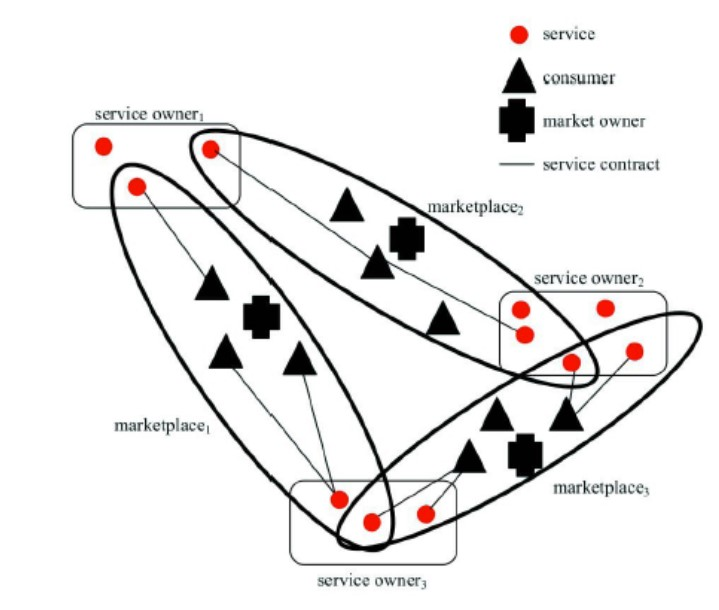
\includegraphics[scale = 0.4]{Images/SOA/WhatIsASOA.jpg}
\end{center}
\end{multicols}

Definizione generale di servizio:
\textbf{funzione, metodo o oggetto con una interfaccia pubblica e stabile, che può essere invocata da un client}. Un servizio può essere considerato come la caratterizzazione astratta e incapsulamento di interfaccia di uno specifico contenuto o risorsa o capacità computazionale (l'abilità di muovere file, creare processi, fornire informazione, ecc\dots).

\subsection{Cos'è una interfaccia di servizio}
Una service interface è definita in termini di protocollo da usare per interagire col servizio, formato di dati scambiati e comportamento previsto dopo che qualche messaggio è stato scambiato. \\

\textbf{Interfaccia} $=$ \textbf{protocollo} $+$ \textbf{formato} $+$ \textbf{comportamento}.\\

Il protocollo dice come interagire col servizio, il formato come i dati scambiati sono strutturati e il comportamento cosa il servizio fa. 

\subsection{Ciclo di vita di un servizio}
\begin{enumerate}
    \item \textbf{Creazione}: il servizio è pubblicato per mezzo di:
    \begin{itemize}
        \item registrazione in una cartella dei servizi (in architetture centralizzate)
        \item disseminazione di messaggi (in architetture decentralizzate)
    \end{itemize}
    \item \textbf{Approvigionamento}: il fornitore e il consumatore stabiliscono un contratto di prestazione di servizi attraverso:
    \begin{itemize}
        \item scoperta: il consumatore trova il servizio più adatto
        \item negoziazione: il contratto è accettato tra le due parti
    \end{itemize}
    \item \textbf{Emanazione}: il servizio è consumato
\end{enumerate}

\subsection{Ruoli partecipanti e interazioni}
SOA è basato su interazioni tra 3 ruoli:
\begin{itemize}
    \item \textbf{Provider}: il possessore del servizio
    \item \textbf{Registry or Broker}: gestisce repositories di informazione sui fornitori e le loro risorse software
    \item \textbf{Consumer}: scopre e invoca risorse software fornite da uno o più providers
\end{itemize}

\subsection{QoS}
A una stessa interfaccia potrebbero corrispondere più implementazioni di servizi, con differenti fornitori e qualità dei servizi. QoS è correlata a aspetti non funzionali che influenzano il modo un servizio è consumato, includendo: performance, disponibilità, robustezza, autorizzazioni richieste, costo. 

Fornitori e consumatori devono stabilire un \textbf{Service Level Agreement (SLA)} che è un accordo QoS. Meccanismi di scoperta sono importanti per permettere ai client di comparare diverse implementazioni di servizi e selezionare la più adatta. 


\chapter{Servizi RESTful}
\section{Introduzione}
REST sta per \textbf{Re}presentational \textbf{S}tate \textbf{T}ransfer e si basa su un protocollo stateless, client$-$server e con comunicazioni memorizzabili. 

Ogni task di gestione dello stato deve essere performato dal client. Piuttosto che protocolli complessi come SOAP per connettere macchine, il semplice \textbf{HTTP} è più frequentemente usato per fare chiamate tra macchine, con server web standard facenti la parte dei server REST. Applicazioni RESTful possono usare richieste HTTP per postare (creare o aggiornare), leggere e eliminare dati. Quindi, applicazioni RESTful possono usare HTTP per tutte le operazioni CRUD (create/read/update/delete). \\

Nonostante sia semplice, REST è completo, non c'è praticamente niente che si possa fare con Web services che non può essere fatto con una architettura RESTful. REST non ha una "standard specification". Non ci sarà mai una raccomandazione di W3C per REST, perchè è uno \textbf{stile architetturale}, non un protocollo.

\subsection{Componenti dell'architettura REST}
\begin{itemize}
    \item \textbf{Risorse}: sono l'elemento chiave di un vero design RESTful. Risorse individuali sono identificate in richieste, per esempio usando URL in sistemi REST web$-$based. Le risorse proprie sono concettualmente separate dalle \textbf{rappresentazioni} che sono ritornate al client. 
    \item \textbf{Una rete di risorse}: significa che una singola risorsa non dovrebbe essere troppo grande e contenere troppi dettagli piccoli. Quando rilevante, una risorsa dovrebbe contenere link a informazioni aggiuntive, come nelle pagine web
    \item \textbf{Non ci sono stati di connessione}: l'interazione è stateless (nonostante il server e le risorse possano essere stateful). Ogni nuova richiesta dovrebbe portare tutte le informazioni richieste per completarla, e non deve affidarsi su interazioni precedenti con lo stesso client. 
    \item Le risposte dovrebbero essere \textbf{memorizzabili (cacheable)} quando possibile (con una data di scadenza). Il protocollo deve permettere al server di specificare esplicatamente quali risposte memorizzare e per quanto.
    \item \textbf{Server proxy}: possono essere usati per come parti di una architettura, per migliorare le performance e la scalabilità. Ogni proxy standard HTTP può essere usato.  
\end{itemize}

\subsection{Servizi RESTful}
Come un web service, un servizio RESTful è:
\begin{itemize}
    \item \textbf{platform-independent}
    \item \textbf{language-independent}
    \item \textbf{standard-based}
\end{itemize}
Come i web services, REST \textbf{non offre funzionalità di sicurezza built-in, cifratura, gestione di sessione, garanzie QoS, ecc\dots}. Ma anche con servizi XML$-$based, questi possono essere aggiunti sopra HTTP:
\begin{itemize}
    \item per la sicurezza, token username/password sono spesso usati
    \item per cifratura, REST può essere usato sopra HTTPS
    \item ecc\dots
\end{itemize}


\section{Esempio: applicazione della rubrica telefonica}
La query probabilmente sarà del tipo:\\

http://www.acme.com/phonebook/user$-$details/12345\\

\'E solo un URI, che è mandato al server usando la semplice richiesta HTTP GET. La risposta HTTP sono i dati grezzi, non inseriti in niente, solo i dati di cui si ha bisogno in un modo che possa usarli direttamente.
Con REST, una semplice connessione di rete è l'unica cosa di cui si ha bisogno. \\

REST può facilmente gestire richieste più complesse, includendo parametri multipli. In molti casi, si useranno i parametri HTTP GET nell'URL. Per esempio:\\

http://www.acme.com/phonebook/user$-$details?name=John\&surname=Doe\\

Se si necessita di passare parametri lunghi, o binari, si usa normalmente la richiesta POST e includere i parametri nel body. 
    
\textbf{Le richieste POST raramente usano XML}. Come mostrato sopra, nella maggior parte dei casi, i parametri di richiesta sono semplici, e non c'è necessità per l'overhead di XML. \textbf{Una risposta del server in REST è spesso un file XML}. Tuttavia, anche altri formati sono usati; diversamente dai servizi SOAP, REST non è connesso a XML in alcun modo. I possibili formati includono \textbf{CSV} e \textbf{JSON}. Ogni formato ha vantaggi e svantaggi:
\begin{itemize}
    \item XML è facile da espandere, e type$-$safe
    \item CSV è più compatto
    \item JSON è banale da analizzare
\end{itemize}

\textbf{Una opzione non è accettabile come formato di risposta REST, eccetto in casi specifici:}
HTML, o qualunque altro formato che è pensato per una comprensione umana e non è facilmente processato dai clients. La eccezione specifica è, ovviamente, quando il servizio REST è documentato per ritornare un documento human$-$readable; e quando vedendo l'intero www come una applicazione RESTful, troviamo che HTML è infatti il formato di risposta REST più comune. 

\section{Routes vs endpoints}
Gli \textbf{endpoint} sono funzioni disponibili attraverso le API. Una \textbf{route} è il nome che si usa per accedere agli endpoint, usato nell'URL. Una route può avere multipli endpoint associati, e quale è usato dipende dal verbo specificato. 

Esempio con l'URL: http://example.com/wp-json/wp/v2/posts/123

\begin{itemize}
    \item La route è wp/v2/posts/123 , non include wp$-$json perchè è il path base per la API stessa
    \item Questa route ha 3 endpoint:
    \begin{itemize}
        \item GET scatena un metodo get\_item, che ritorna i dati post al client
        \item PUT scatena un metodo update\_item, che prende i dati da aggiornare e ritorna i dati post aggiornati
        \item DELETE scatena un meteodo delete\_item, che ritorna i dati post eleminati ora al client
    \end{itemize}
\end{itemize}

\begin{center}
    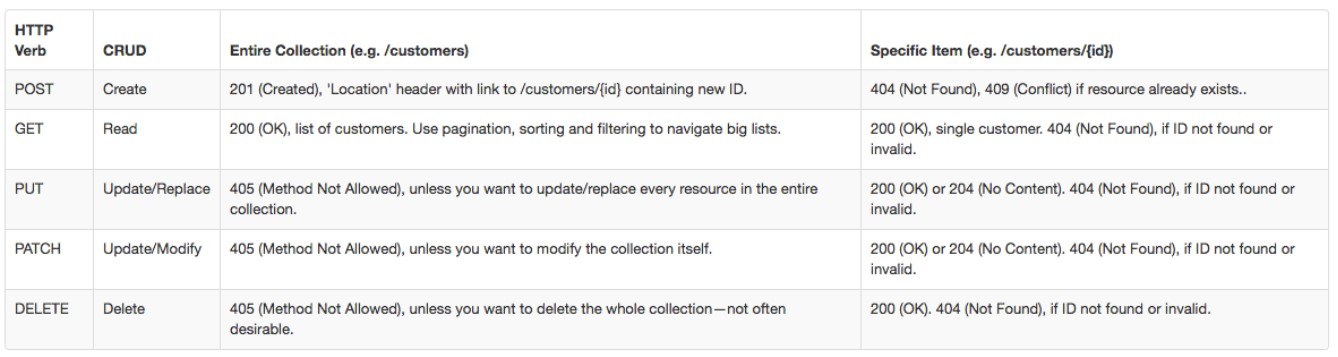
\includegraphics[scale = 0.4]{Images/SOA/HTTP.jpg}
\end{center}

\section{Linee guida progettazione REST}
\begin{enumerate}
    \item \textbf{Non usare URL fisici}: un URL fisico punta a qualcosa di fisico ad esempio un file XML: "http://www.acme.com/inventory/product003.xml" mentre un URL logico non indica un file fisico: "http://www.acme.com/inventory/products/003". Anche con l'estensione xml il contenuto potrebbe essere generato dinamicamente ma dovrebbe essere umanamente visibile che l'URL è logico e non fisico.
    
    \item \textbf{Le query non dovrebbero tornare un sovraccarico di dati}
    \item \textbf{Anche se la risposta REST può essere tutto, assicurarsi che sia ben documentata}, e non cambiare il formato di output di poco. Se l'output è XML, bisogna assicurarsi di documentarlo con uno schema o DTD.
    \item \textbf{Piuttosto che permettere che i client costruiscano URL per azioni aggiuntive, includere gli URL e le risposte REST}. 
\end{enumerate}


\chapter{Microservizi}
\section{Il monolite}
Quando tutte le funzionalità di un sistema devono essere implementate insieme, viene considerato un \textbf{monolite}.

In un \textbf{monolite monoprocesso}, tutto il codice è contenuto in un singolo processo. Il \textbf{monolite modulare} è una variazione in cui il processo singolo consiste di moduli separati. Si può lavorare su ognuno in modo indipendente, ma tutti necessitano di essere combinati insieme per l'implementazione. Un \textbf{monolite distribuito} è un sistema che consiste in servizi multipli, ma per qualche ragione, il sistema intero deve essere implementato insieme.


\section{Cosa sono i microservizi}
I microservizi sono servizi rilasciabili in modo indipendente che sono modellati su un dominio di business. Un servizio incapsula funzionalità e le rende accessibili ad altri servizi esponendo uno o più endpoint di rete (una cosa o una API REST).

\begin{center}
    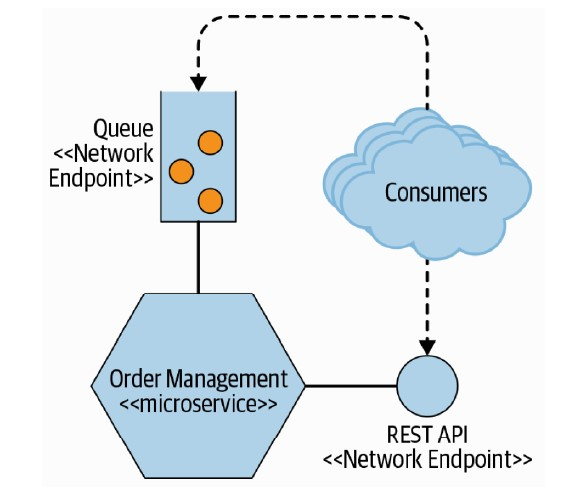
\includegraphics[scale = 0.4]{Images/SOA/WhatAreMicroservices.jpg}
\end{center}

\emph{“The microservice approach has emerged from real-world
use, taking our better understanding of systems and
architecture to do SOA well. You should think of
microservices as a specific approach for SOA in the same
way that Extreme Programming (XP) or Scrum are
specific approaches for Agile software development.”}\\

Dall'esterno, un singolo servizio è trattato come una \textbf{black box}, nascondendo il più possibile ed esponendo il meno possibile tramite interfacce esterne. I dettagli implementativi interni sono interamente nascosti dal mondo esterno. Ciò significa che le architetture di microservizi \textbf{evitano di usare database condivisi} nella maggior parte delle circostanze; invece, ogni microservizio incapsula il suo database proprio dove richiesto.

Avere \textbf{limiti di servizio chiari e stabili} che non cambiano quando
le modifiche di implementazione interna si traducono in sistemi che hanno
\textbf{accoppiamento più lasco} e \textbf{coesione più forte}.\\

\textbf{Implementabilità indipendente} è l'idea che si può fare un cambiamento a un microservizio, implementarlo, e rilasciare quel cambiamento all'utente, senza aver bisogno di implementare un altro servizio. 
\begin{multicols}{2}
\textbf{Modellando servizi per un dominio di business} possiamo facilitare la pubblicazione di nuove funzionalità, e facilitare la ricombinazione di microservizi in modi diversi per portare nuove funzionalità agli utenti.
\begin{center}
    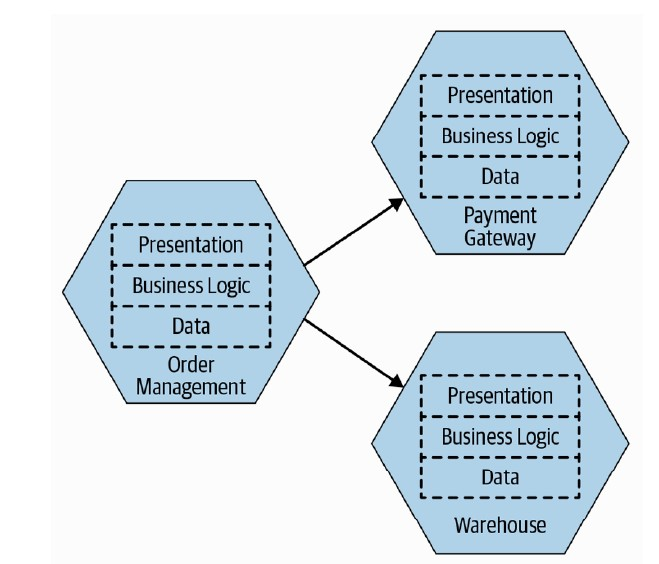
\includegraphics[scale = 0.4]{Images/SOA/WhatAreMicroservices2.jpg}
\end{center}
\end{multicols}
Quanto grande dovrebbe essere un microservizio? Non c'è una risposta ultima a questa domanda, dovrebbero avere una interfaccia la più piccola possibile. Tuttavia, avere troppi microservizi troppo piccoli potrebbe risultare in un incremento della complessità del sistema e richiedere nuove skill e tecnologie.

Un vantaggio principale dei microservizi è che suportano una \textbf{eterogeneità delle tecnologie}. Si possono prendere gli strumenti corretti per ogni implementazione di servizio. Si può facilmente cambiare tecnologia di un microservizio, senza affliggere gli altri microservizi.
\begin{center}
    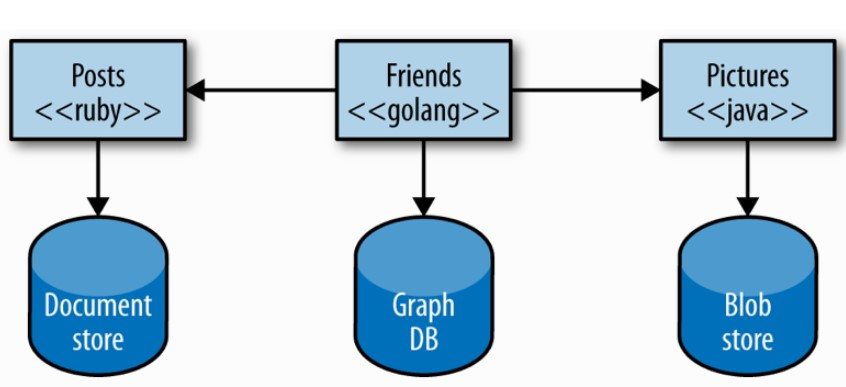
\includegraphics[scale = 0.4]{Images/SOA/WhatAreMicroservices3.jpg}
\end{center}

\section{Come modellare i microservizi}
Usare il \textbf{dominio} come meccanismo primario per identificare confini dei microservizi è la soluzione migliore in generale. 
\subsection{Coesione}
Si vogliono le funzionalità raggruppate in modo tale che si possano fare modifiche in meno posti possibili.

\subsection{Accoppiamento debole}
Lo scopo dei microservizi è quello di essere in grado di fare un cambiamento a un servizio e implementarlo, senza necessità di cambiare altre parti del sistema.

\subsection{Accoppiamento di dominio}
\textbf{Accoppiamento di dominio} descrive la situazione dove un microservizio necessita di interagire con un altro microservizio, perchè deve usare una funzionalità che l'altro fornisce.
\begin{center}
    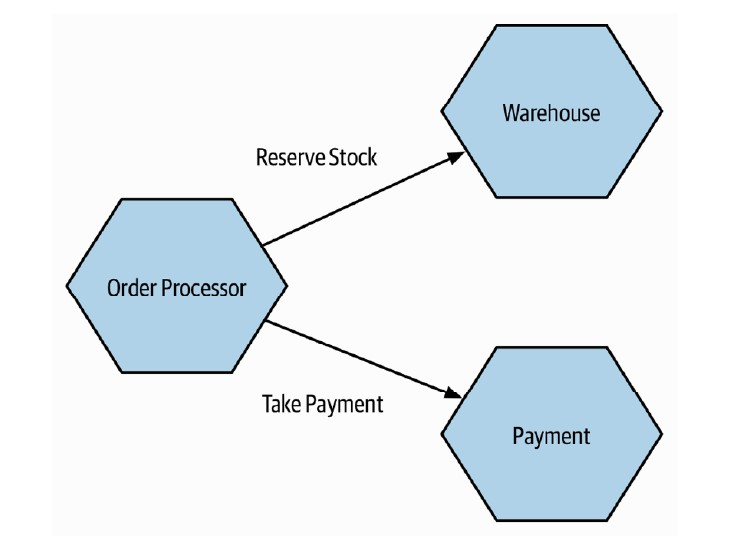
\includegraphics[scale = 0.4]{Images/SOA/ModelMicroservices.jpg}
\end{center}

\subsection{Passare attraverso l'accoppiamento}
Descrive una situazione in cui uno
il microservizio passa i dati a un altro microservizio esclusivamente perché esso
è necessario per qualche altro microservizio a valle.
\begin{center}
    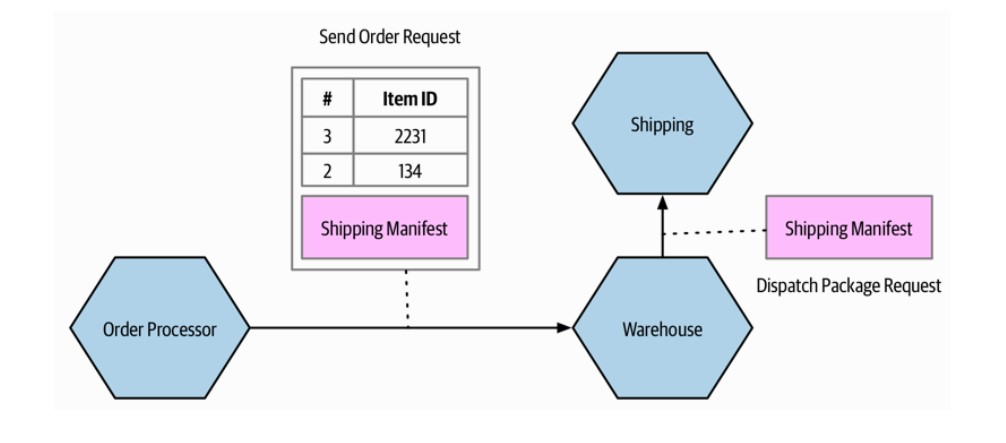
\includegraphics[scale = 0.4]{Images/SOA/ModelMicroservices2.jpg}
\end{center}
Il problema principale con l'accoppiamento pass-through è che una modifica ai dati richiesti a valle può causare una modifica a monte più significativa.

Soluzione 1: comunicare direttamente col servizio a valle
\begin{center}
    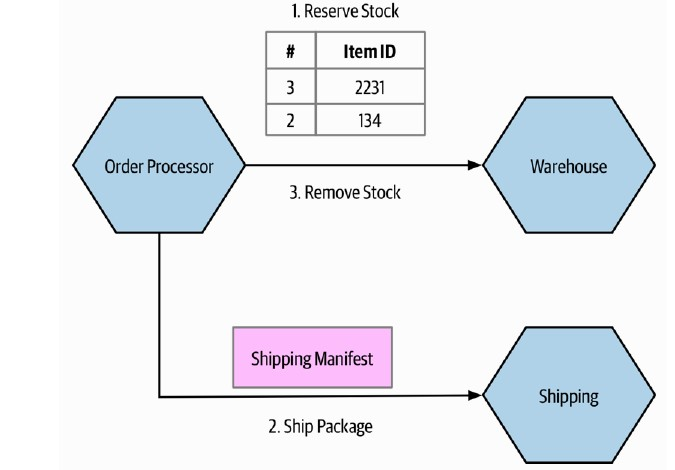
\includegraphics[scale = 0.4]{Images/SOA/ModelMicroservices3.jpg}
\end{center}

Soluzione 2: evita la propagazione non necessaria di messaggi
\begin{center}
    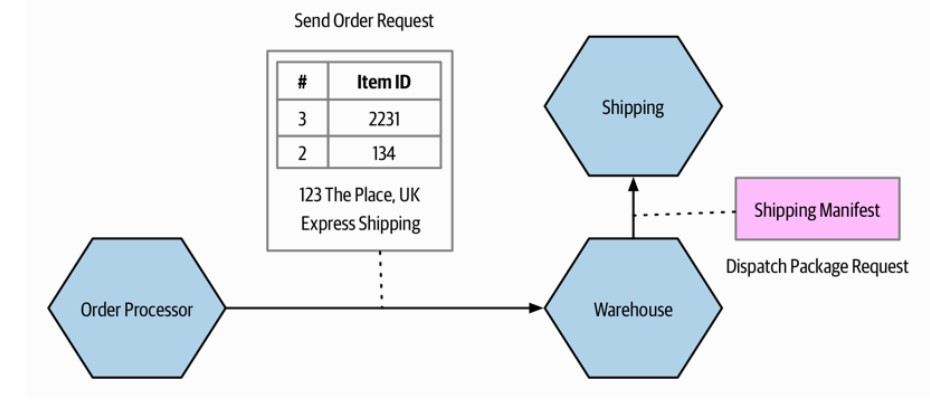
\includegraphics[scale = 0.4]{Images/SOA/ModelMicroservices4.jpg}
\end{center}


\subsection{Accoppiamento comune}
Avviene quando due o più microservizi fanno uso di un set comune di dati. Si deve evitare di usare lo stesso database.
\begin{center}
    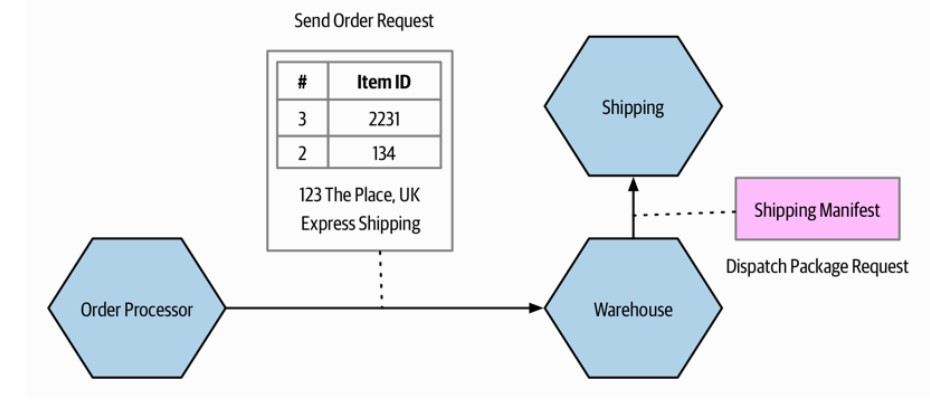
\includegraphics[scale = 0.4]{Images/SOA/ModelMicroservices4.jpg}
\end{center}
La natura dei dati che si stanno mantenendo e gestendo può portare a diversi forme di decomposizione:
\begin{center}
    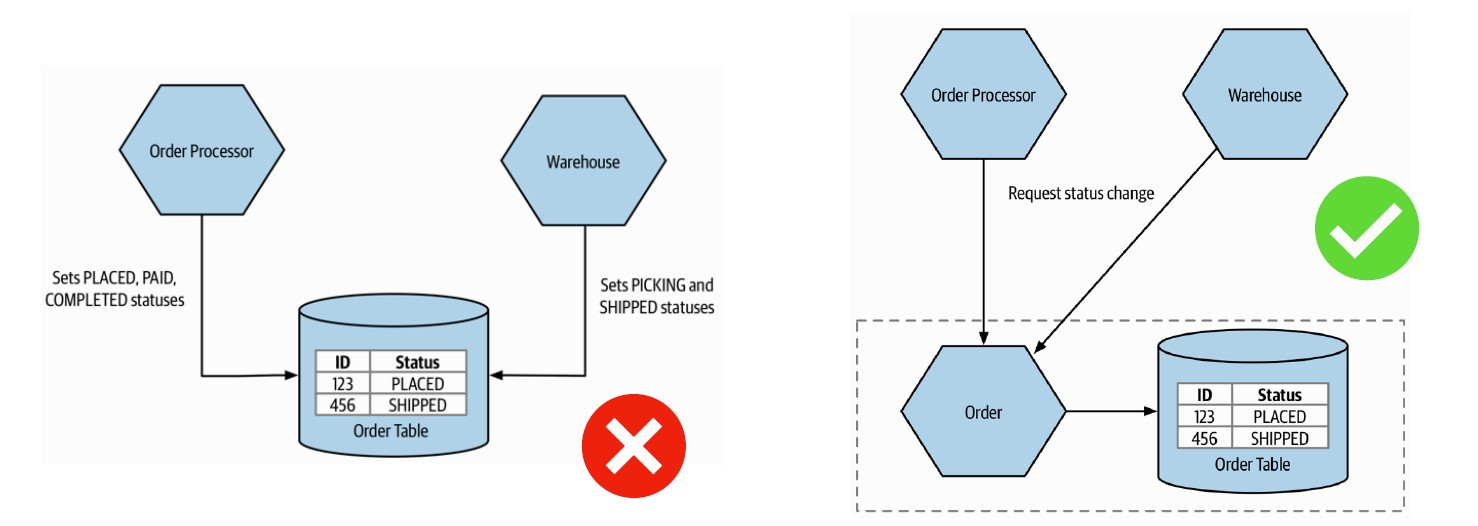
\includegraphics[scale = 0.4]{Images/SOA/ModelMicroservices5.jpg}
\end{center}

\section{Stili di comunicazione dei microservizi}
\begin{center}
    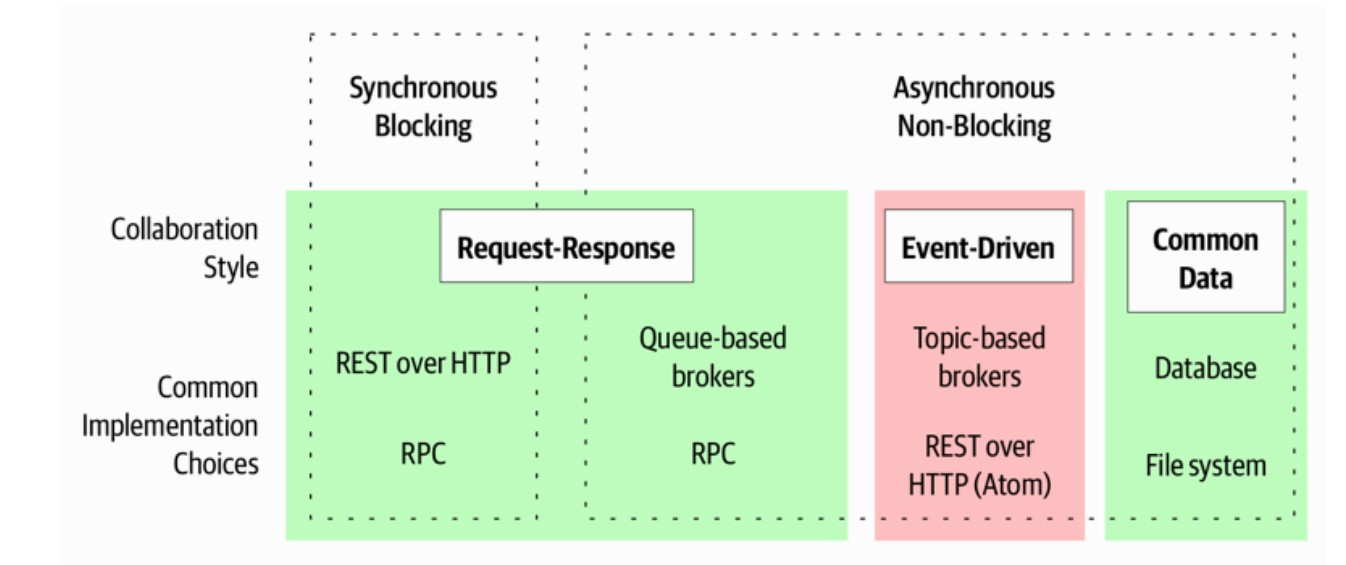
\includegraphics[scale = 0.4]{Images/SOA/MicroservicesCommunicationStyles.jpg}
\end{center}
\begin{itemize}
    \item \textbf{Synchronous Blocking}: un microservizio fa una chiamata a un altro microservizio e blocca le operazioni aspettando la risposta
    \item \textbf{Asynchronous Non-Blocking}: il microservizio che emette una chiamata è in grado di portare avanti l'elaborazione indipendentemente da se la chiamata è ricevuta o no
    \item \textbf{Request-Response}: un microservizio manda una richiesta ad un altro chiedendo che qualcosa venga eseguito. Si aspetta di ricevere una risposta alla richiesta che informa del risultato
    \item \textbf{Event-Driven}: i microservizi emettono eventi, che gli altri consumano e reagiscono secondo le regole. Il microservizio che emette l'evento non è consapevole di quale microservizio consuma gli eventi che emette
    \item \textbf{Common Data}: i microservizi collaborano tramite qualche sorgente dati condivisa
\end{itemize}

\subsection{Implementare la comunicazione tra microservizi}
Tecnologie:
\begin{itemize}
    \item \textbf{Remote Procedure Calls} (le chiamate a metodi locali sono invocate da un processo remoto)
    \begin{itemize}
        \item SOAP
        \item gRPC
        \item CORBA
    \end{itemize}
    \item \textbf{REST} (risorse accedute tramire metodi semplici HTTP)
    \item \textbf{GraphQL} (query personalizzate possono ricavare informazioni da multipli microservizi a valle)
    \item \textbf{Message Brokers} (middleware per comunicazione asincrona sia via code che topics)
\end{itemize}

Per comunicazioni richiesta$-$risposta: gRPC, REST, GraphQL.\\
Per comunicazioni asincrone: message brokers 
\begin{center}
    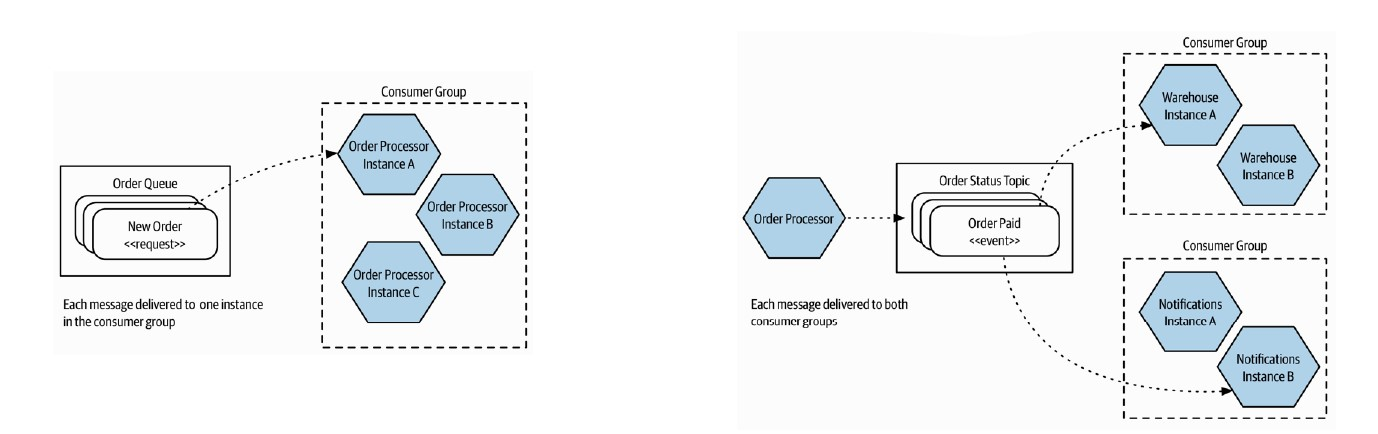
\includegraphics[scale = 0.4]{Images/SOA/ImplementingMicroserviceComm.jpg}
\end{center}

\section{Workflow}
\textbf{Anti-Pattern}: Algoritmo di commit a due fasi
\begin{center}
    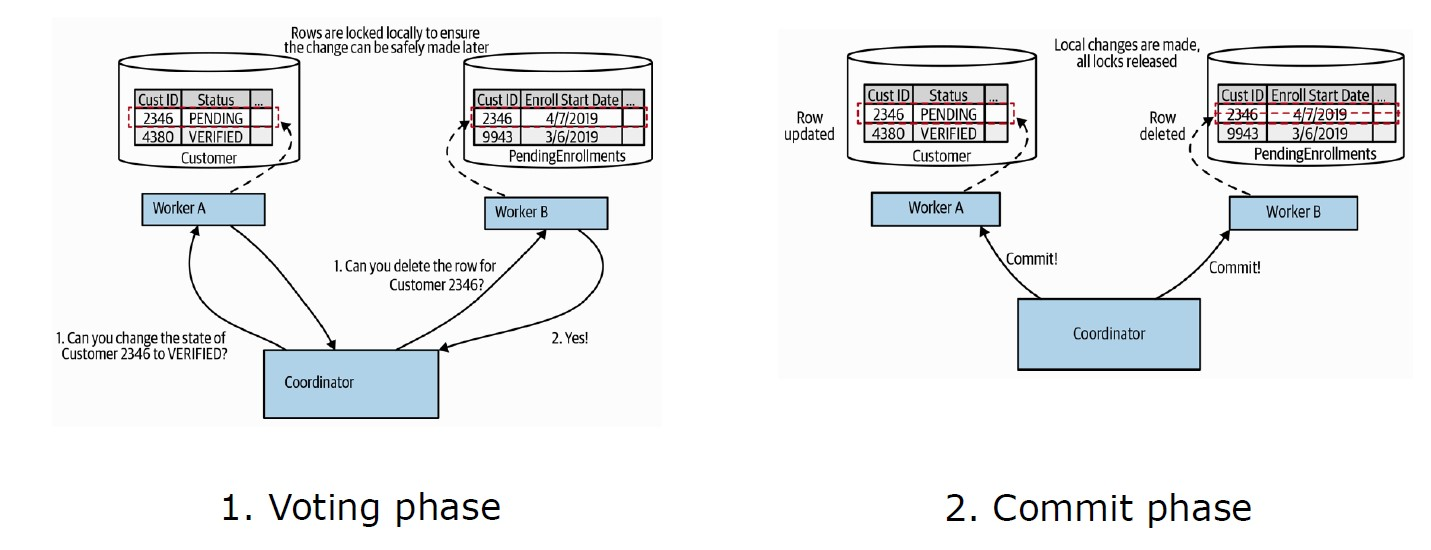
\includegraphics[scale = 0.4]{Images/SOA/WorkFlow.jpg}
\end{center}
L'algoritmo qua sopra (e in generale le transazioni distribuite) \textbf{deve essere evitato} perchè possono essere un modo veloce per introdurre una grande quantità di latenza nel sistema. 
\begin{center}
    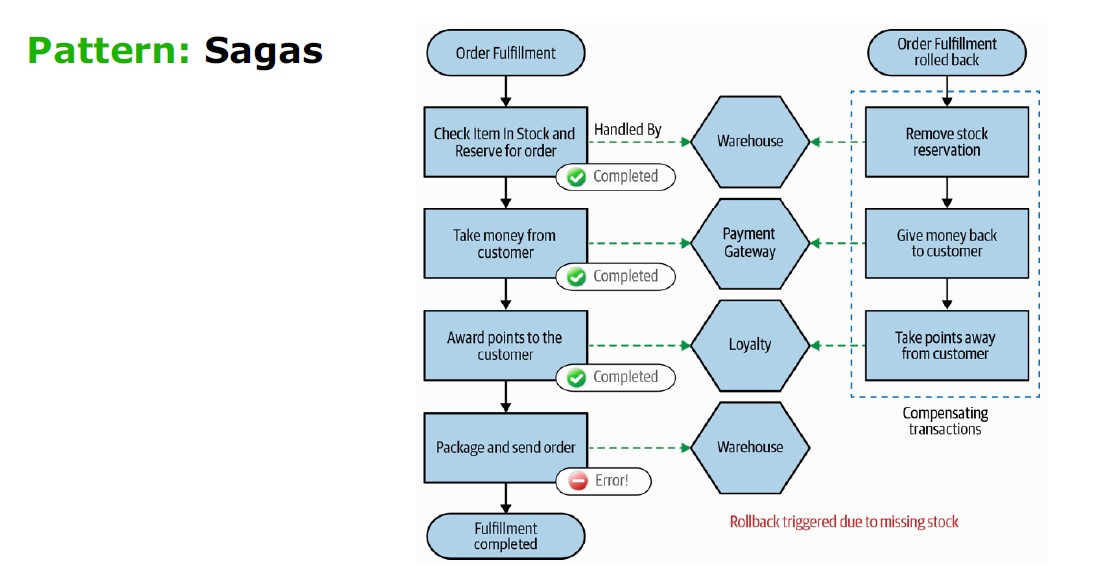
\includegraphics[scale = 0.4]{Images/SOA/PatternSagas.jpg}
\end{center}

\section{Costruzione}
\subsection{Continuous Integration (CI)}
Assicurati che il codice appena registrato si integri correttamente con
codice esistente. Per fare ciò, un server CI rileva che il codice è stato eseguito,
lo controlla ed esegue alcune verifiche come assicurarsi
il codice viene compilato e i test passano.
Come minimo, ci aspettiamo che questa integrazione venga eseguita su a
quotidianamente.
Evitare l'uso di rami di lunga durata per lo sviluppo di funzionalità e
considera invece lo \textbf{sviluppo basato su trunk}. Se proprio devi usare i rami, tienili corti!

\subsection{Build pipelines and continuous delivery}
Avere diversi stage nella costruzione. Ottienere feedback costanti sulla prontezza di produzione di ogni checkin. Inoltre, trattare ogni checkin come un candidato per la release:
\begin{center}
    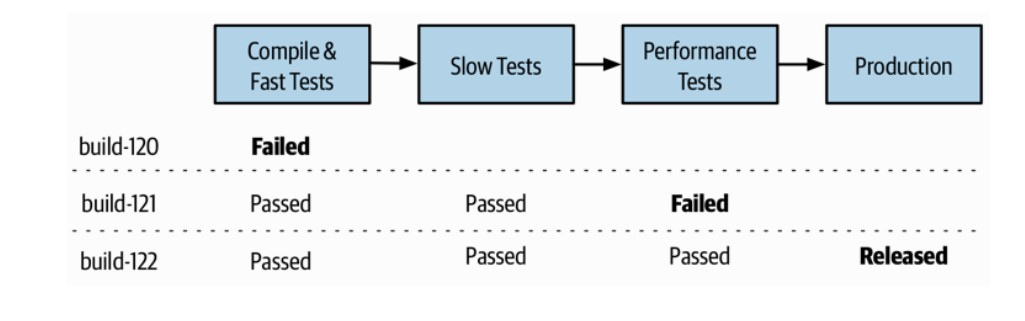
\includegraphics[scale = 0.4]{Images/SOA/Build.jpg}
\end{center}

\subsection{One repository per microservice (aka multi-repo)}
Il codice sorgente per ogni microservizio è memorizzato in una repository di codice sorgente separata. Si deve avere il codice che si vuole riutilizzare contenuto in una libreria che poi diventa una dipendenza esplicita a valle dei microservizi.
\begin{center}
    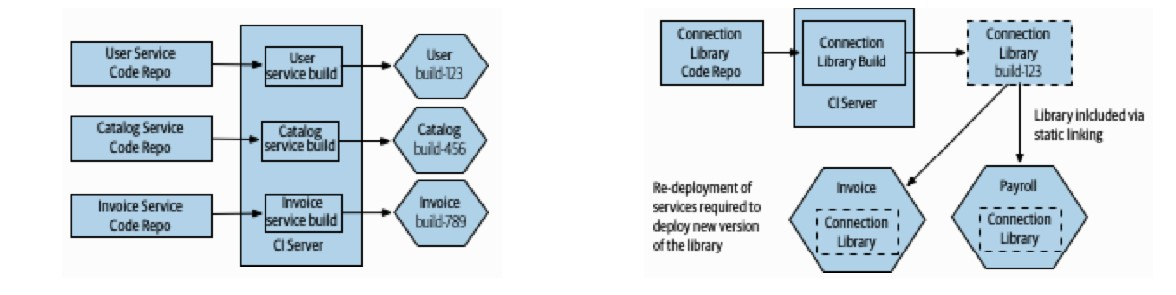
\includegraphics[scale = 0.4]{Images/SOA/MultiRepo.jpg}
\end{center}

\section{Implemenetazione}
Implementazione di database e ridimensionamento
\begin{center}
    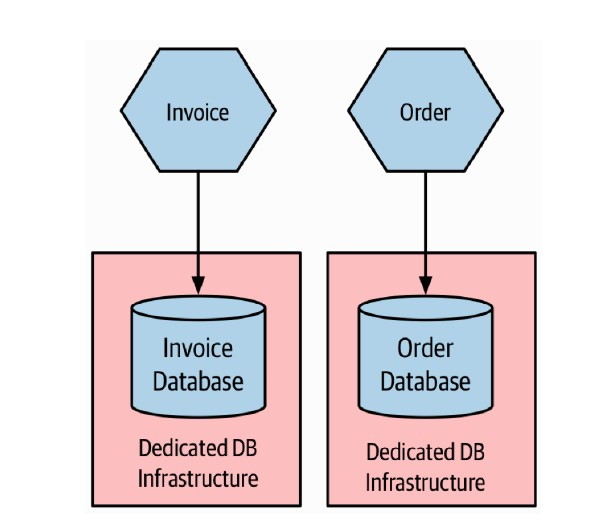
\includegraphics[scale = 0.4]{Images/SOA/Deployment.jpg}
\end{center}

Ambienti diversi per parti differenti della pipeline
\begin{center}
    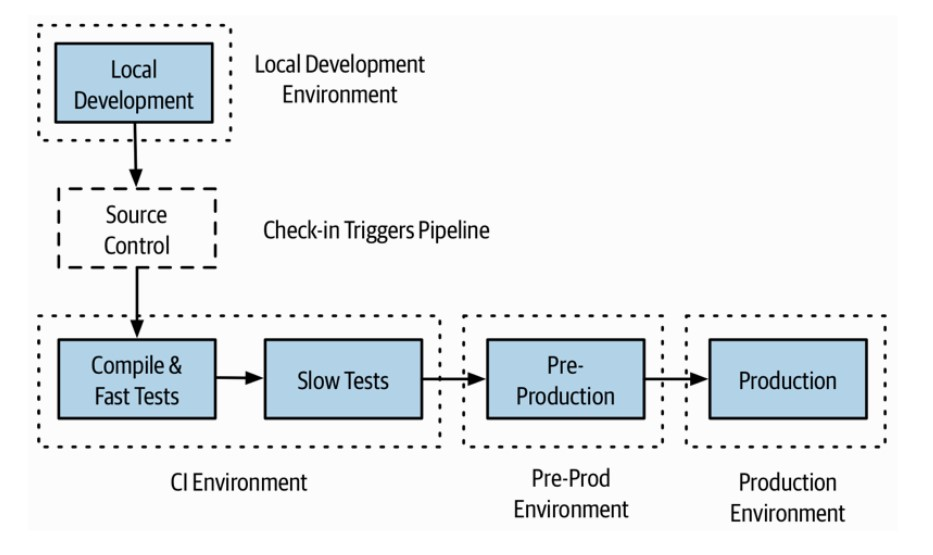
\includegraphics[scale = 0.4]{Images/SOA/Deployment2.jpg}
\end{center}
Principi dell'implementazione di microservizi
\begin{itemize}
    \item \textbf{Esecuzione isolata}
    \item \textbf{Concentrazione sull'automazione}
    \item \textbf{Infrastruttura come codice}
    \item \textbf{Implementazione a zero tempo di inattività}
    \item \textbf{Gestione dello stato desiderato}
\end{itemize}

\begin{multicols}{2}
Opzioni di implementazione:
\begin{itemize}
    \item Macchina fisica
    \item Macchina virtuale
    \item Container
    \item Applicazione container
    \item Platform as a service (Heroku, Google App Engine)
    \item Function as a service (AWS Lambda, Azure Cloud Functions)
\end{itemize}
\begin{center}
    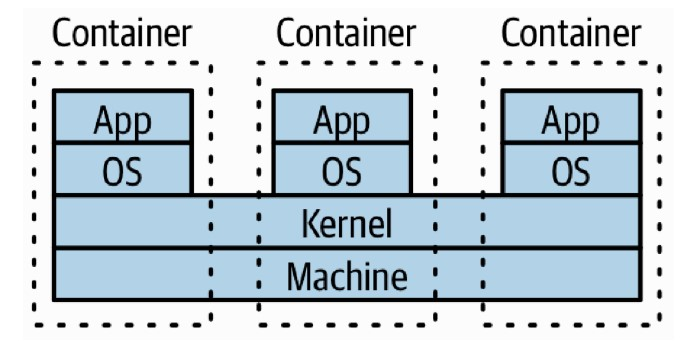
\includegraphics[scale = 0.4]{Images/SOA/Deployment3.jpg}
\end{center}

\end{multicols}

Esecuzione di microservizi in container separati:
\begin{center}
    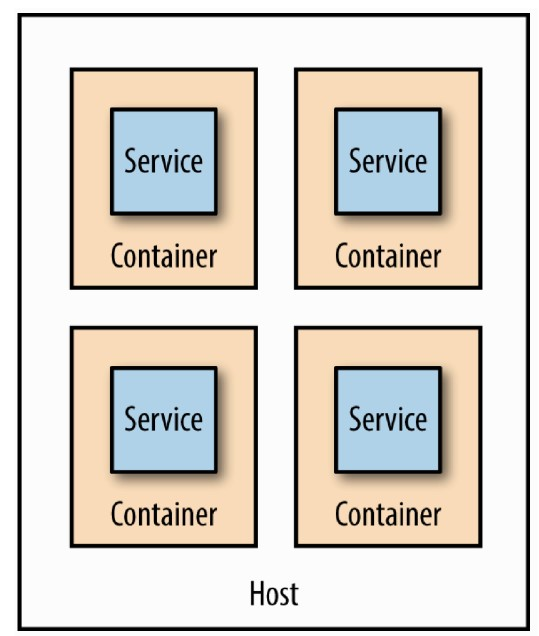
\includegraphics[scale = 0.4]{Images/SOA/Deployment4.jpg}
\end{center}

Molteplici microservizi per applicazioni container:
\begin{center}
    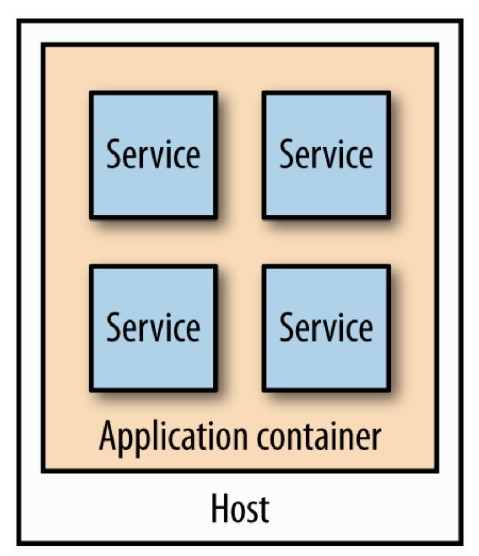
\includegraphics[scale = 0.4]{Images/SOA/Deployment5.jpg}
\end{center}



